\chapter{Micro-architecture}
We have designed and written the RTL in Chisel \cite{10.1145/2228360.2228584} domain-specific language or DSL. Chisel is a DSL embedded in Scala programming languages. It allows for easy integration to Chipyard for different purposes such as FireSim \cite{8416816} simulations, VLSI integration, and FPGA targets. 
\section{Chisel API}
The APIs are implementation of common hardware constructs provided to us by Chipyard \cite{chipyard} and Chisel \cite{Asanović:EECS-2016-17} and the team of Chipyard developers.

We have used Chisel constructs in our design to implement common hardware blocks. A queue is an example of such constructs that are provided by Chisel. 
\begin{verbatim}
val reqQueue = Module(new Queue(new MainQueue(geom, tlParams),
                                geom.QUEUEDEPTH, pipe=false))    
\end{verbatim}
The code above instantiates a simple queue that stores the requests entering the memory controller data path. The reqQueue elements then can be accessed using the I/O ports of the Queue module. The Queue module provides a ready-valid interface on both enqueue and dequeue sides. When there is a new request, the request bundle can be stored using the API as shown below:
\begin{verbatim}
    when (io.frontReq.fire) {
      reqQueue.io.enq.valid := true.B
      reqQueue.io.enq.bits.we := io.frontReq.bits.isWrite
      reqQueue.io.enq.bits.addr := io.frontReq.bits.address
      reqQueue.io.enq.bits.cmdID := id
      reqQueue.io.enq.bits.bankNo := io.frontReq.bits.bankNo
      reqQueue.io.enq.bits.byteEnable := io.frontReq.bits.byteEnable
      reqQueue.io.enq.bits.requesterID := io.frontReq.bits.requesterID
    }
\end{verbatim}

The when construct corresponds to a combinational logic always block in Verilog. The code above uses methods defined in the IO class such as fire. Fire is the event that both ready and valid are high for an interface. This style of coding makes it easier and faster to write the RTL. 

Using standard Scala functional programming features such as \verb|.filter()|, \verb|.foreach()|, and \verb|.tabulate()| helped us write the RTL more concisely while maintaining code readability. 

Packets in Chisel can be constructed by creating a class that extends the Bundle class of Chisel. A bundle is a group of directional wires that have the same context. In our case, we standardized all of our bundle classes to contain output wires. In case a bundle is used as an input to a module, a \verb|Bundle| can be used to flip all the directions for that bundle. An example bundle usage in our RTL is the input to the Bank Machines described in Chapter \ref{chap:arch}. The bank input packet includes a field for write or read, address, id, and mask. If the transaction is a write transaction, the write enable field or \verb|we| is true and the byte enable is used to mask the write data. 
\begin{verbatim}
class BankInPacket (val geom : GeomParams) extends Bundle {
  val we         = Output(Bool())
  val addr       = Output(UInt((geom.FULLADDRBITS).W))
  val cmdID      = Output(UInt((geom.IDBITS).W))
  val byteEnable = Output(UInt((geom.TLBYTEEN).W))
}
\end{verbatim}
Using this bundle as an input port to the Bank Machine module is done through a Decoupled interface which adds ready and valid signals to the bundle. 
\begin{verbatim}
class BankMachine (val geom : GeomParams, val bankNo : Int) extends Module {
  val io = IO(new Bundle {
    val in = Flipped(Decoupled(new BankInPacket(geom)))
    ...
\end{verbatim}
The in field of the IO port in a Bank Machine is a decoupled, flipped bundle of \verb|BankInPacket|. The \verb|Decoupled| makes the IO port a decoupled interface with ready and valid signals. The ready signal is set by the consumer of this packet which is the Bank Machine module, and the valid signal is asserted by the producer of the signal which is the data path module. A \verb|io.in.fire| event corresponds to the transfer of the packet from the producer to the consumer. 
\section{Datapath Micro-architecture}
The datapath in our design refers to the module that takes in requests from the TileLink module and keeps track of the transactions and the data. As an example, a write request must be kept in the data path until the write transaction is ready to be issued to DFI. At that point, the data can be taken out of the memory controller and sent to the DFI. 
The data path has two main modules within it, a read queue module, and a write queue module. The read, and write queues keep the data in 8 banks of SRAMs.
The data path interfaces to the top module of the memory controller. The top module connects the ports from the data path to the DFI read and write interface. The top module connects the data path to its input ports which are connected to the TileLink front module. Figure \ref{fig:data_uarch} shows the micro-architecture diagram of the data path. The data path has an internal counter for ID assignment to transactions. This counter is by default a 10-bit counter but can be configured to a wider counter to avoid ID collisions. Each TileLink request that is captured by the TileLink module first is synchronized to the controller clock frequency and then enters the data path module where it is assigned an ID. If the transaction is a write transaction, then the data path must store the data with the corresponding ID in the write queue SRAMs. The depth of the write queue SRAMs indicates the maximum write requests that can be in flight at any point. However, the request queue which stores both read and write transactions provided a ready signal to the SoC. The designer of the SoC must size the request queue to be equal to or greater than the write or read queues. 

A capturing logic is implemented in the data path to capture a read response from the DFI. Once a read response arrives, the DFI packet asserts a read data valid signal. The data is delivered to DFI on PHY clock frequency which is four times faster than the controller clock. DFI delivers the data to the memory controller per cycle using four phase scheme. On each cycle, data is split into four phases of 32 bits that are delivered over 2 cycles which make up the 256-bit total data width of the controller. The read data capturing waveform is shown in Figure \ref{fig:read-cap}.

A similar logic is in place to stream the write data from a 256-bit wide register to the DFI over two cycles.  Figure \ref{fig:write-trans} shows the transmission of the write data to DFI. 
\begin{figure}
    \centering
    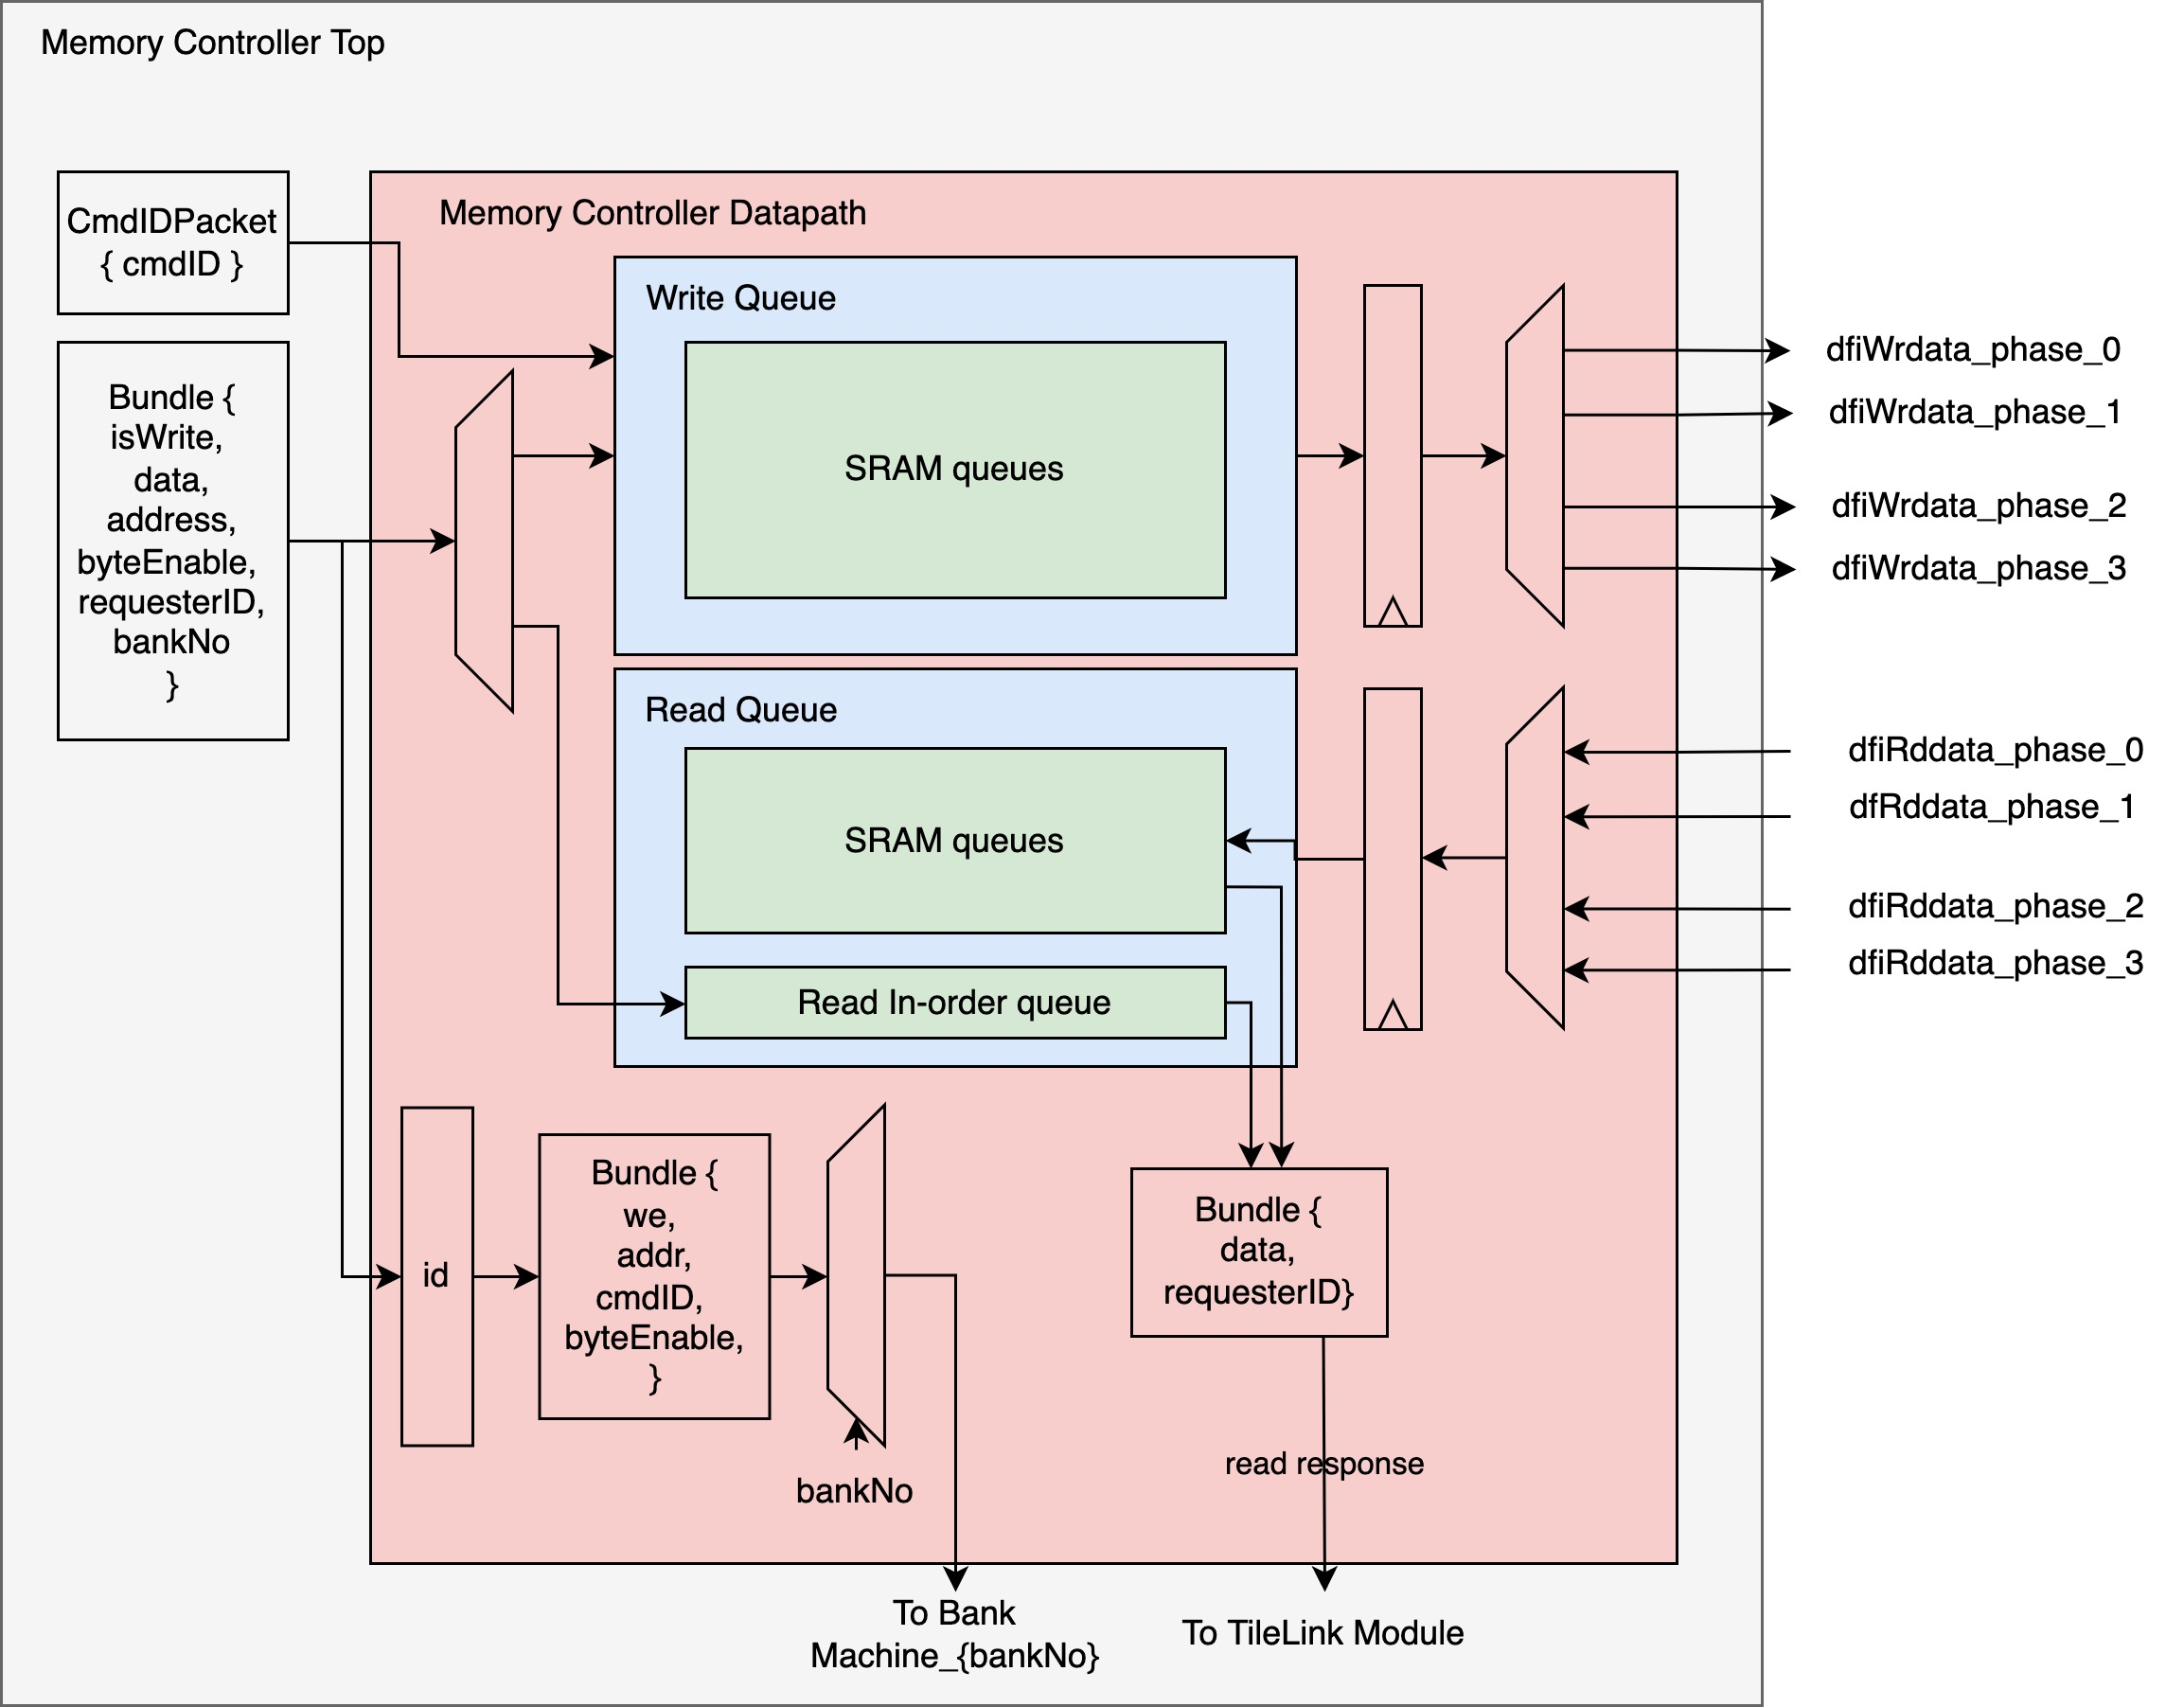
\includegraphics[scale=0.2]{images/datapath-u.jpg}
    \caption{Datapath internal logic.}
    \label{fig:data_uarch}
\end{figure}
\begin{figure}
    \centering
    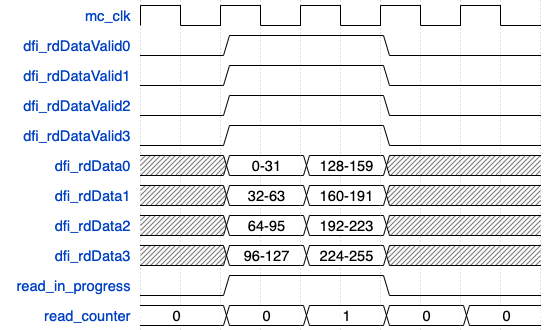
\includegraphics[scale=0.5]{images/read-capture.png}
    \caption{Capturing of DFI read response.}
    \label{fig:read-cap}
\end{figure}
\begin{figure}
    \centering
    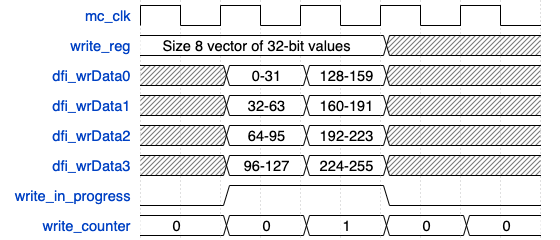
\includegraphics[scale=0.5]{images/writes-to-dfi-mod.png}
    \caption{Transmission of DFI write data.}
    \label{fig:write-trans}
\end{figure}
\newpage
\section{TileLink Lazy Module}
TileLink elaboration depends on a lazy system to connect the nodes together and avoid a deadlock in the bus system. A TileLink node would be instantiated in the system at the time of elaboration. In case there are mismatches between the bus width, the TileLink diplomacy monitors' assertions would stop the compilation process. The deadlock-free requirements are also checked at the compile time. Our design relies on API provided by Diplomacy to create a manager node as well as a register node in the TileLink lazy module.

The manager node connects to the Memory Bus of the system and accepts packets on channel A of TileLink. We have designed our manager node to be compatible with the TL-UL protocol. TL-UL is a TileLink Uncached Lightweight protocol that requires channel A and D implementations. Data in the DRAM is not cached and as a result, the TileLink node for the memory controller does not need to implement channels B and C. The controller manager node for the controller can only accept packets that are one beat only. In large SoC with wider bus widths, TileLink adopts a multi-beat packet protocol. In such systems, a \verb|Fragmenter| module is instantiated automatically to translate the multi-beat packets to one packet and vice versa. The \verb|Fragmenter| takes in as input a multi-beat packet and once the packet is fully transmitted, sends the constructed one-beat packet to the controller. It can also perform the same logic in the opposite direction where the controller can produce a one-beat packet and send it to the \verb|Fragmenter|, which internally breaks up the packet into a multi-beat packet.

\section{Synthesis Result}
We synthesized the design as part of our initial assessment phase of the tape-out process using Hammer, a physical design flow tool \cite{10.1145/3489517.3530672}. The reports are based on Intel 16 technology which is a 22 nm FinFET process node. The synthesis report indicates a relatively small area footprint. The synthesis report in table \ref{tab:syn_report} shows the instance types used from the technology library.

In table \ref{tab:area}, the subsequent area report shows a breakdown of our memory controller by modules. Note that all area units are in micro-meter squared.
\begin{table}[H]
    \centering
    \begin{tabular}{c|c|c|c}
         Type & Instances & Area & \% Area  \\
         \hline
         Sequential & 6973 & 9529 & 64.9 \\
         Inverter & 897 & 183 & 1.2 \\
         Buffer & 39 & 35.109 & 0.2 \\
         Clock Gate & 420 & 657 & 4.5 \\
         logic & 10022 & 4284  & 29.2 \\
         total & 18351 & 14690 & 100.0 \\
    \end{tabular}
    \caption{Synthesis report.}
    \label{tab:syn_report}
\end{table}

\begin{table}[H]
    \centering
    \begin{tabular}{c|c|c|c}
    Instance & Module & Cell Count & Total Area \\
    \hline
    top & MemoryControllerTop & 18351 & 18961.802 \\
    core & MemoryControllerCore & 8759 & 8371.554 \\ 
    datapath & MemoryControllerDataPath & 9128 & 10099.057\\
    \end{tabular}
    \caption{Area breakdown by module.}
    \label{tab:area}
\end{table}